\documentclass[12pt, oneside]{article} 
\usepackage{amsmath, amsthm, amssymb, calrsfs, wasysym, verbatim, bbm, color, graphics, geometry}

\geometry{tmargin=.75in, bmargin=.75in, lmargin=.75in, rmargin = .75in}  
\setlength{\parindent}{0in}
\setlength{\parskip}{\baselineskip}%
\setlength{\parindent}{1.5pt}%

\newcommand{\R}{\mathbb{R}}
\newcommand{\C}{\mathbb{C}}
\newcommand{\Z}{\mathbb{Z}}
\newcommand{\N}{\mathbb{N}}
\newcommand{\Q}{\mathbb{Q}}
\newcommand{\Cdot}{\boldsymbol{\cdot}}
\newcommand{\block}[1]{
  \underbrace{\begin{matrix}1 & \cdots & 1\end{matrix}}_{#1}
}
\newtheorem{thm}{Theorem}
\newtheorem{defn}{Definition}
\newtheorem{conv}{Convention}
\newtheorem{rem}{Remark}
\newtheorem{lem}{Lemma}
\newtheorem{cor}{Corollary}
\usepackage{tikz}  %TikZ central library is called.
\usetikzlibrary{automata,positioning} 
\usepackage{standalone}
\usepackage{pdfpages}

\tikzset{%
  every neuron/.style={
    circle,
    draw,
    minimum size=0.8cm
  },
  neuron missing/.style={
    draw=none, 
    scale=2,
    text height=0.2cm,
    execute at begin node=\color{black}$\vdots$
  },
  arro/.style={
    ->,
    >=latex
  },
  bloque/.style={
    draw,
    minimum height=1cm,
    minimum width=0.5cm
  }  
}


\title{Lecture Note - 07: Neural Network}
\author{Dihui Lai}

\begin{document}

\maketitle
\tableofcontents

\vspace{.25in}

\section{A Single Neuron}

An artificial neuron is the basic computing unit in an artificial neural network. There are different way to define a neuron. The most common one is shown in Figure 1.
\begin{figure}
\center
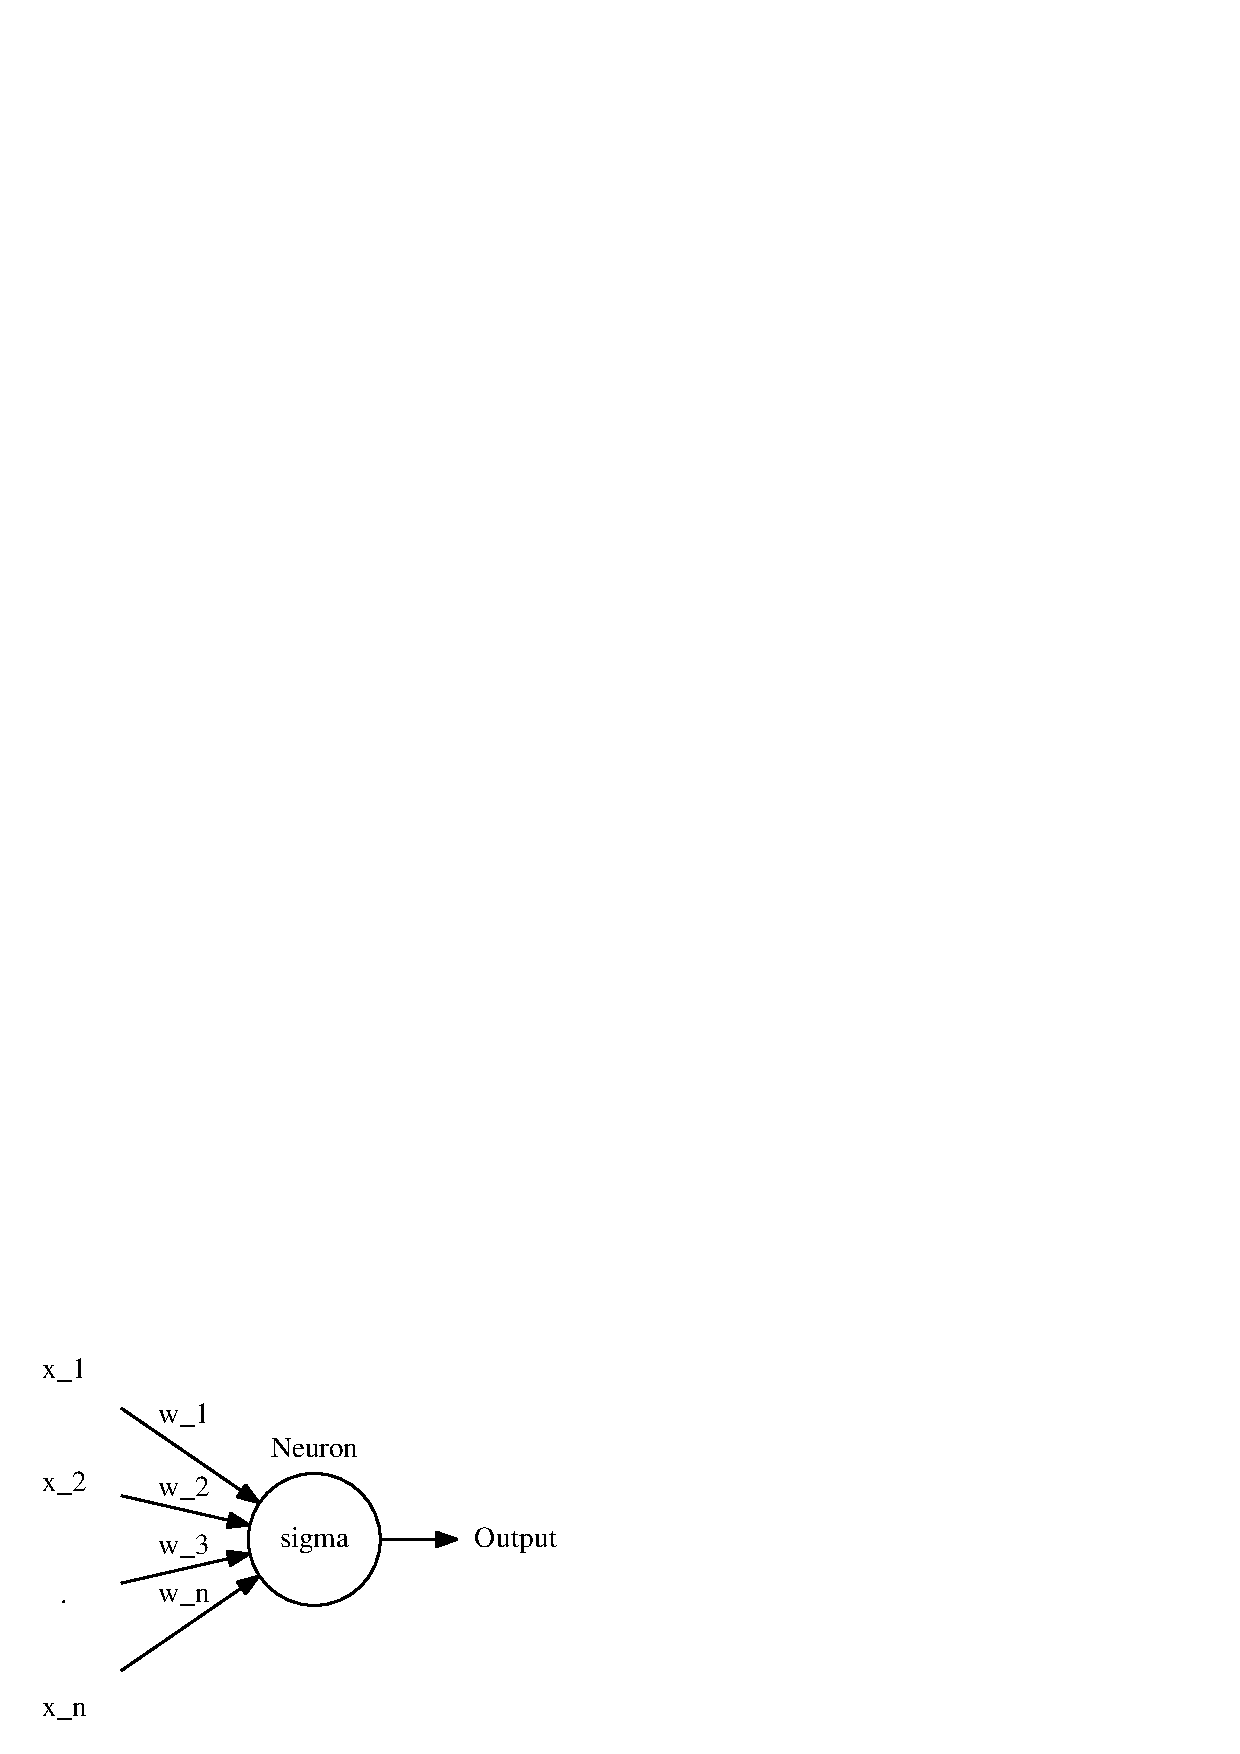
\includegraphics[scale=0.6,page=1]{Figures/singleneuron.pdf}
\caption{Schema: a single neuron with activation function $\sigma$}
\end{figure}

\textbf{Input}: A neuron receives multiple inputs $x_1$, $x_2$, ..., $x_n$. The signals are summed up after modulated by a set of weights $w_1$, $w_2$, ... $w_n$. Let us denote the weighted sum $z$
\begin{equation}
z=\sum\limits_{i=1}^{n}w_i x_i
\end{equation}

Usually a biased term $w_0$ is added to the summation and we have 
\begin{equation}
z=\sum\limits_{i=1}^{n}w_i x_i+w_0
\end{equation}

\textbf{Output}: The weighted sum is further transferred via an activation function $\sigma$ and becomes the final output of the neuron
\begin{equation}
o=\sigma(z)=\sigma(\sum\limits_{i=1}^{n}w_i x_i+w_0)
\end{equation}

\textbf{Activation}: The activation function can of different types.  Below is a list of common activation functions. Almost all activation functions have an S-shape except for the ReLu function.
\begin{center}
\bgroup
\def\arraystretch{2.5}% 
\begin{tabular}{c|c} 
Name & Definition\\
\hline
Step Function & $\sigma (z)={\begin{cases}0&{\text{for }}z<0\\1&{\text{for }}z\geq 0\end{cases}}$\\
\hline
Logistic or sigmoid & $\sigma(z)={\frac {1}{1+e^{-z}}}$\\
\hline
hyperbolic tangent &$\sigma(z)={\frac {(e^{z}-e^{-z})}{(e^{z}+e^{-z})}}$\\
\hline
ReLU & $\sigma(z)=\begin{cases}0&{\text{for }}z\leq 0\\z&{\text{for }}z>0\end{cases}$
\end{tabular}
\egroup
\end{center}


\section{Neural Network}
\begin{figure}
\includestandalone[width=.8\textwidth]{Figures/neuralnetwork}
\caption{A neural network of multiple layer structures. The hidden layers before layer $l-1$ and after layer $l$ are not shown. }
\end{figure}




\end{document}

